% Compile using: TEXINPUTS=minted/source: xelatex -shell-escape slides.tex
\documentclass[14pt,compress,english,utf8,t]{beamer}

\usepackage{etex}

\usepackage[english]{babel}

\usepackage{tikz}
\usepackage{booktabs}
\usepackage{ragged2e}
\usepackage[normalem]{ulem}

\makeatletter
\ifbeamer@draftmode
\usepackage{verbatim}
\newcommand{\inputminted}[2]{\verbatiminput{#2}}
\else
\usepackage{minted}
\setminted{linenos}
\fi
\makeatother

\usetikzlibrary{calc,shapes.callouts,shapes.arrows}
\definecolor{darkred}{RGB}{220,0,0}
\newcommand{\hcancel}[5]{%
    \tikz[baseline=(tocancel.base)]{
        \node[inner sep=0pt,outer sep=0pt] (tocancel) {#1};
        \draw[darkred, line width=1mm] ($(tocancel.south west)+(#2,#3)$) -- ($(tocancel.north east)+(#4,#5)$);
    }%
}%

\usepackage[protrusion=true,expansion=false]{microtype}

\usepackage{fontspec}
\newfontfamily\DejaSans{DejaVu Sans}

\title[
  \raisebox{-0.3mm}{\DejaSans ☺} Perl 6 is out for your enjoyment
  \raisebox{-0.3mm}{\DejaSans ☺}
]{\raisebox{-0.3mm}{\DejaSans ☺} Perl 6 \raisebox{-0.3mm}{\DejaSans ☺} \\
  is out for your enjoyment
}
\author[Ingo Blechschmidt]{\small Ingo Blechschmidt}
\institute{32th Chaos Communication Congress}
\date[December 30th, 2015]{\small December 30th, 2015}

\usetheme{Warsaw}
\usecolortheme{seahorse}
\definecolor{mypurple}{RGB}{150,0,255}
\setbeamercolor{structure}{fg=mypurple}
\usefonttheme{serif}
\usepackage{fontspec}
\defaultfontfeatures{Mapping=tex-text}
\setmainfont{Linux Libertine O}
\useinnertheme{rectangles}
\setbeamercovered{invisible}

\setbeamertemplate{title page}[default][colsep=-1bp,rounded=false,shadow=false]
\setbeamertemplate{frametitle}[default][colsep=-2bp,rounded=false,shadow=false,center]

\setbeamertemplate{navigation symbols}{}
\setbeamertemplate{headline}{}

\newcommand*\oldmacro{}%
\let\oldmacro\insertshorttitle%
\renewcommand*\insertshorttitle{%
  \oldmacro\hfill\insertframenumber\,/\,\inserttotalframenumber\hfill}

\newcommand{\hil}[1]{{\usebeamercolor[fg]{item}{\textbf{#1}}}}

\newcommand{\atpos}[1]{%
  \begin{tikzpicture}[remember picture, overlay]%
    \node[anchor=south east] at (current page.south east) {#1};
  \end{tikzpicture}%
}

\newcommand{\centeredpar}[2]{%
  \begin{center}
    \colorbox{white}{\parbox{#1\textwidth}{%
      #2%
    }}%
  \end{center}%
}

\newcommand{\sourcedquote}[4]{%
  ``#1''\par%
  {\raggedleft -- #2, #3, \href{#4}{\underline{link}}\par}%
}

% Gonzalo Medina, http://tex.stackexchange.com/a/228198
\makeatletter
\def\Mdescription#1{%
  \advance\beamer@descdefault by \labelsep%
  \list
  {}
  {\labelwidth\beamer@descdefault%
  \leftmargin\beamer@descdefault%
  \let\makelabel\beamer@descriptionitem
  \settowidth\labelwidth{\beamer@descriptionitem{#1}}%
  \setlength\leftmargin{\labelwidth}% 
  \addtolength\leftmargin{\labelsep}%
  }%
  \beamer@cramped%
  \raggedright
  \beamer@firstlineitemizeunskip%
}
\def\endMdescription{\ifhmode\unskip\fi\endlist}
\long\def\beamer@descriptionitem#1{%
  \def\insertdescriptionitem{#1}%
  {\usebeamertemplate**{description item}}\hfil}
\makeatother

\setbeameroption{show notes}
\setbeamertemplate{note page}[plain]

\begin{document}

\begin{frame}
  \titlepage

  \vspace*{-1em}
  \begin{center}
    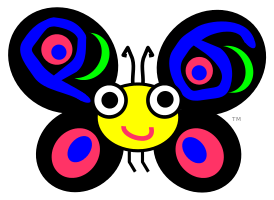
\includegraphics[scale=0.40]{images/camelia}
  \end{center}
\end{frame}

\begin{frame}[plain,c]
  \hspace*{-0.4cm}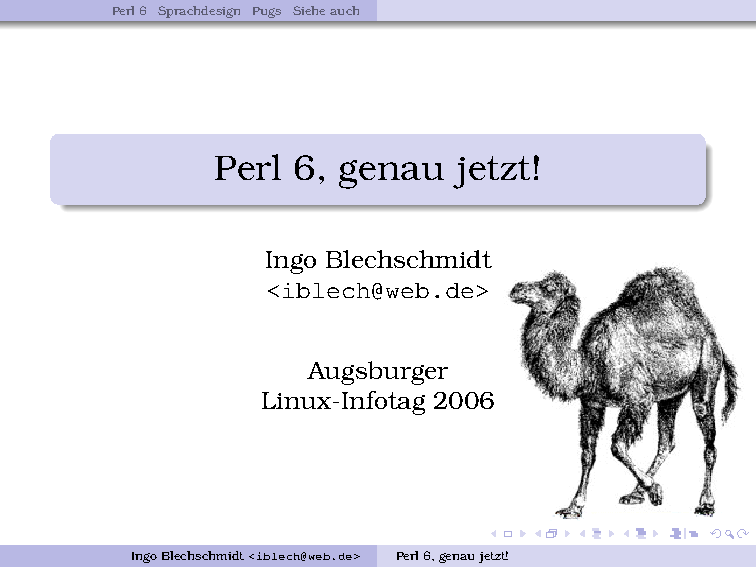
\includegraphics[page=1,scale=0.9]{images/Perl6_LIT_2006.pdf}
\end{frame}

\begin{frame}[plain,c]
  \centering
  
\includegraphics[scale=0.6]{images/happy-camel.jpeg}
  \par
\end{frame}

\begin{frame}[plain,c]
  \centering
  
\includegraphics[scale=0.4]{images/applause}
  \par
\end{frame}

\begin{frame}\frametitle{Perl 6 \ldots}
  \begin{itemize}
    \item is a modern programming language
    \item is a reimagination of Perl 5
    \item is expressive
    \item is multi-paradigmatic
    \item has dramatically overhauled regexes
    \item is fully Unicode-aware
    \item has vast meta-programming abilities
  \end{itemize}
\end{frame}

\begin{frame}[fragile]\frametitle{Example 1}
  \begin{minted}{perl}
class SmilingCat is Cat {
    has Double $.smiling-power = 9000;

    method smile(Person $to, Bool $jump?) {
        say "Hello $to!";
        say "I'm jumping!" if $jump;
        $to.happiness += self.smiling-power;
                       # or $.smiling-power
    }
}
  \end{minted}
\end{frame}

\begin{frame}[fragile]\frametitle{Example 2}
  \begin{minted}{perl}
a
  \end{minted}
\end{frame}

% http://www.impactlab.net/wp-content/uploads/2010/09/Happy-Camel-672.jpg
% http://cdn.theatlantic.com/static/mt/assets/science/bender-applause_medium.gif

\end{document}
